%-------------------------
%big-picture
%(c) H.Buchmann FHNW 2008
%$Id$
%export TEXINPUTS=${HOME}/fhnw/edu/:${HOME}/fhnw/edu/tinL/config/latex:${HOME}/fhnw/edu/config//:
%-------------------------
\documentclass{beamer}
\usepackage{latex/beamer}
%---------------------
%local defines
%(c) H.Buchmann FHNW 2009
%$Id$
%---------------------
\newcommand{\target} {\beaglebone\xspace}
\newcommand{\targetS}{{\bf BBG}\xspace}
\newcommand{\host}   {{\em Host}\xspace}
\newcommand{\targetroot} {{\bf target-root}\xspace}
\newcommand{\kernel} {{\bf kernel}\xspace}
\renewcommand{\c}{{\bf C}\xspace}
\newcommand{\cpp}{{\bf C++}\xspace}
\newcommand{\posix}{{\bf POSIX}\xspace}


\title[Netzwerk]{Netzwerk}
\begin{document}

\frame{\titlepage}

\begin{frame}{Ziel}{\target am Schulnetz}
 \begin{itemize}
  \item Verschiedene Netze
  \begin{itemize}
   \item {\em Schulnetz} passwortgeschützt
   \item {\em lokales Netz} \host{} \target 
  \end{itemize}
  \item Gesucht
  \begin{itemize}
   \item Verbindung {\em Schulnetz} $\leftrightarrow$ {\em lokales Netz}
  \end{itemize}
  \item Wichtiger Begriff
  \begin{description}
   \item[Proxy] Stellvertreter
  \end{description}
  \item Was wir möchten
  \begin{itemize}
   \item \cod{HTTP} auf \target
   \item \cod{apt-get ...}
  \end{itemize}
 \end{itemize}
\end{frame}

\begin{frame}{Zwei Netze}{zwei Rechner}
 \begin{center}
 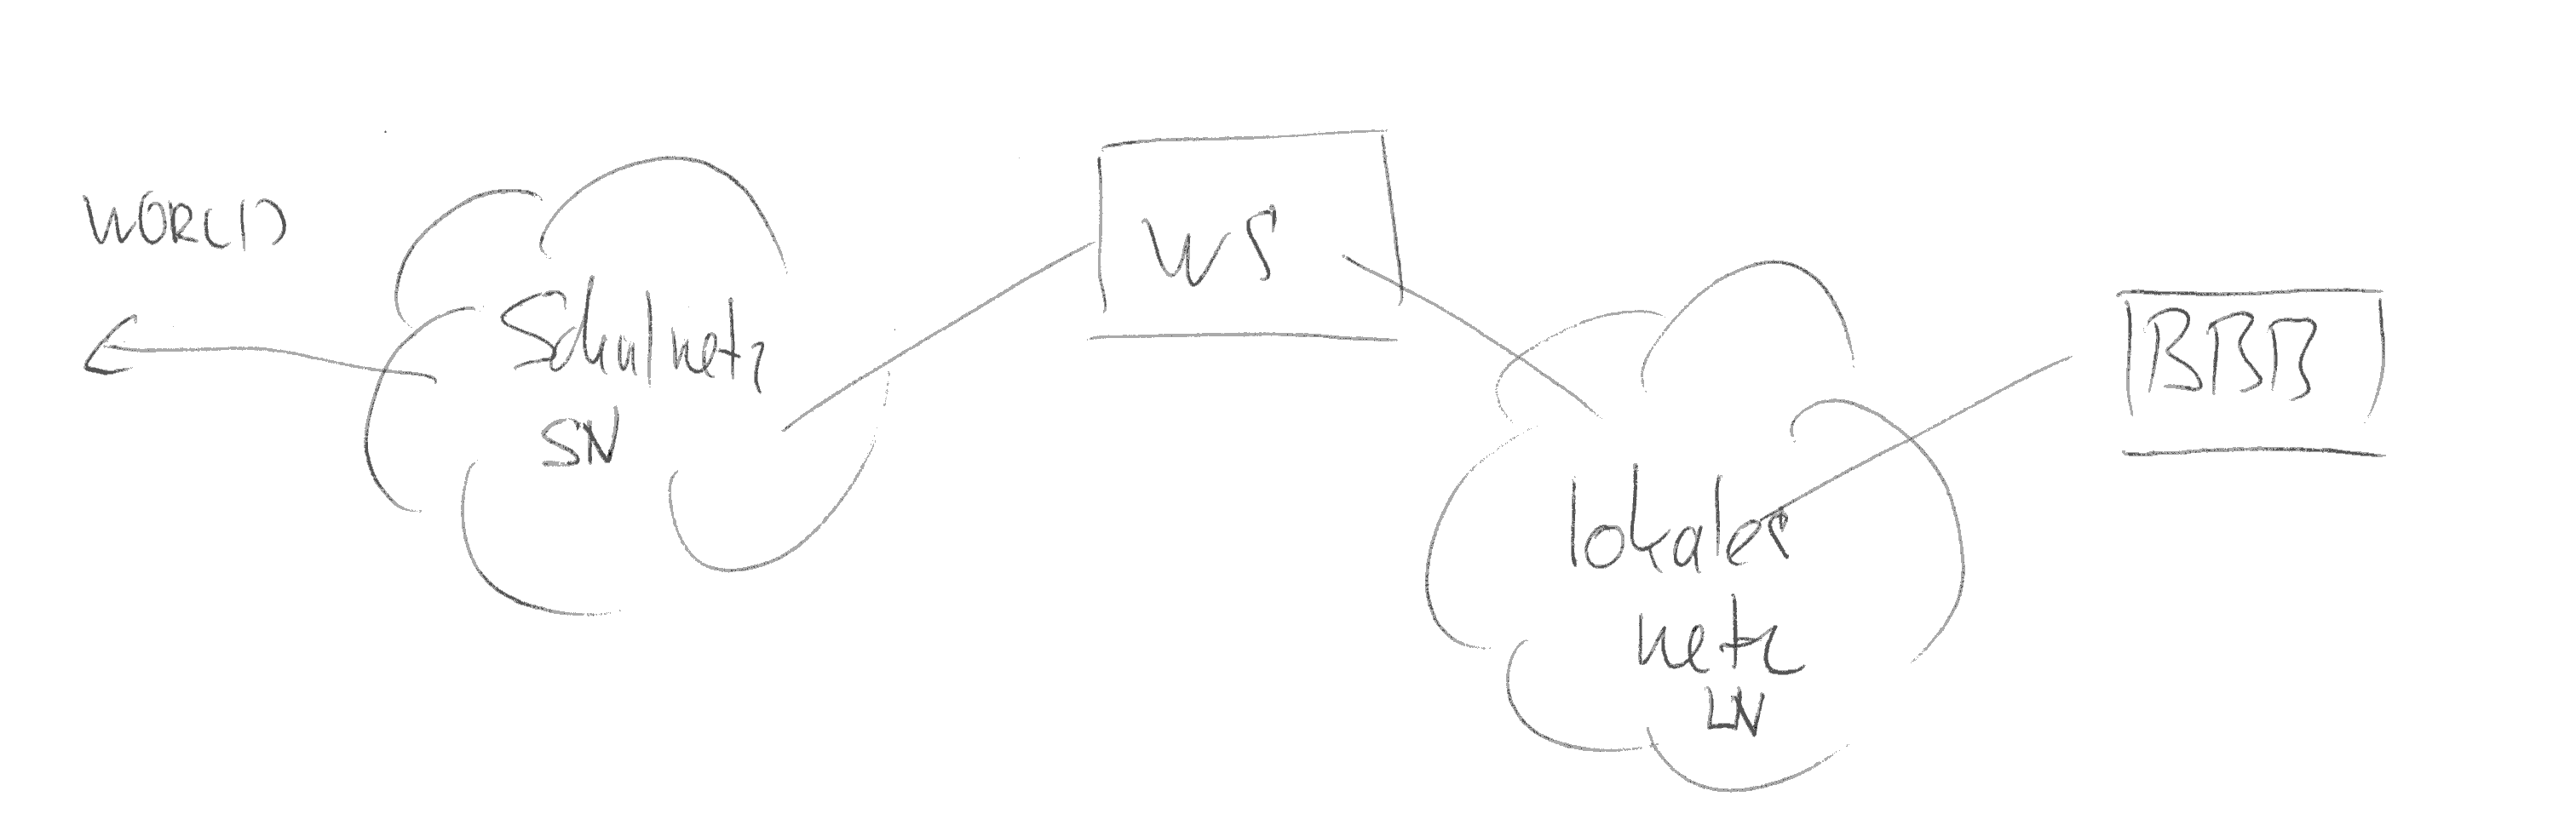
\includegraphics[width=0.875\textwidth]{two-networks.png}
 \end{center}
 \begin{itemize}
  \item Netze
  \begin{description}[LokalesNetz (LN)]
  \item[Schulnetz   (SN)] {\em mit} Verbindung zum Internet
  \item[LokalesNetz (LN)] {\em ohne} Verbindung zum Internet
  \end{description}
  \item Rechner
  \begin{description}[\target(BBB)]
   \item[Workstation(WS)] am SN und LN
   \item[\target(BBB)] am LN  
  \end{description}
 \end{itemize}
\end{frame}

\section{HTTT Proxy}

\begin{frame}{Proxy}{Stellvertreter}
  \begin{center}
 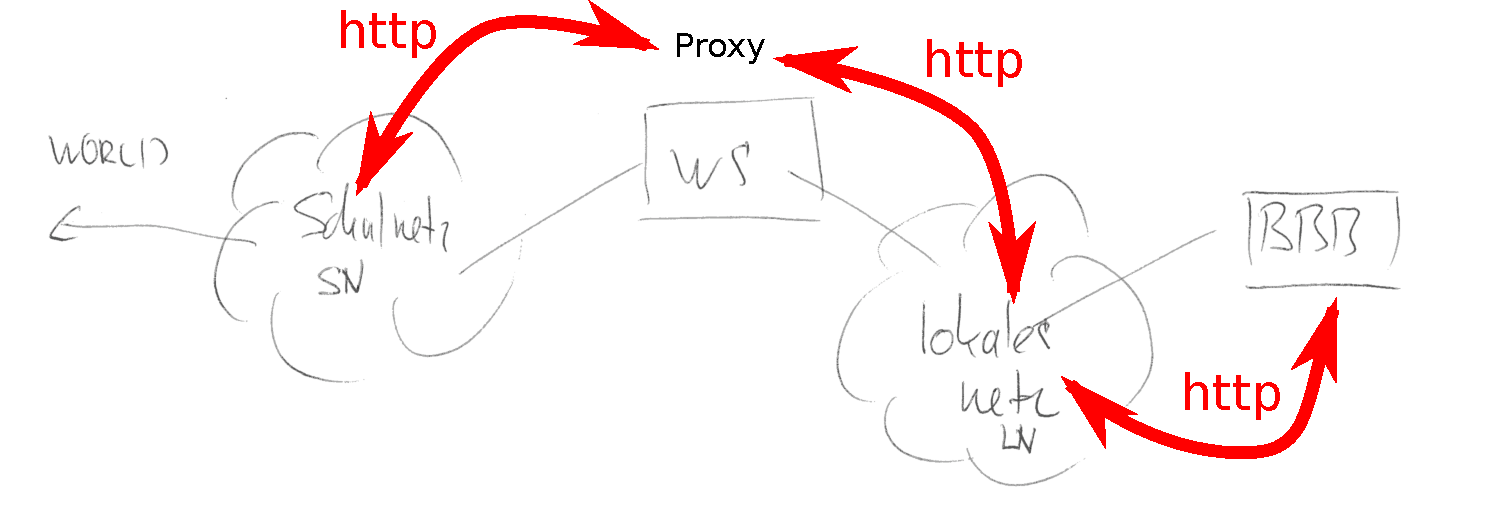
\includegraphics[width=0.875\textwidth]{proxy.pdf}
 \end{center}
 \vspace{-1.5cm}
 \begin{itemize}
  \item Server auf \host
  \item reicht die \cod{http} {\em requests/responses} weiter
 \end{itemize}
 \remark{funltioniert nur f�r \cod{http}}
\end{frame}

\begin{frame}{Test mit \cod{curl}}{\url{curl.haxx.se/}}
  \begin{itemize}
   \item \cod{curl address}
   \begin{itemize}
    \item \cod{curl fhnw.ch}
    \item \cod{curl -v address} \cod{-v}: verbose
   \end{itemize}
  \end{itemize}
\end{frame}

\begin{frame}{Proxy Server}{drei Vorschl�ge}
 \begin{itemize}
  \item \cod{tinyproxy}
  \vspace{-5mm}
  \begin{quote}
  lightweight http(s) proxy daemon
  \end{quote}
  \begin{itemize}
   \item {\scriptsize\url{tinyproxy.github.io}}
  \end{itemize}
  \item \cod{polipo}
   \vspace{-5mm}
   \begin{quote} 
   is a lightweight caching and forwarding web proxy server
   \end{quote}
%   \vspace{-5mm}
   \begin{itemize}
    \item {\scriptsize\url{www.pps.univ-paris-diderot.fr/~jch/software/polipo/}}
   \end{itemize}
  \item \cod{squid}
   \vspace{-5mm}
   \begin{quote} 
   is a caching proxy for the Web supporting
   \end{quote}
   \begin{itemize}
     \item {\scriptsize\url[http]{www.squid-cache.org/}}
   \end{itemize}
 \end{itemize}
\end{frame}


\begin{frame}{\cod{tinyproxy}}{direkter Aufruf}
 \begin{description}[\target]
  \item[\host] Skript Server
  \begin{itemize}
   \item \cod{./tools/tinyproxy.sh}
  \end{itemize}
  \item[\target] Client
  \begin{itemize}
   \item \cod{curl --proxy http://192.168.7.1:8888  \textbackslash\\ www.google.ch}
  \end{itemize}
 \end{description}
 \remark{Wie steht es mit \cod{https}}
\end{frame}

\begin{frame}{\target}{\cod{apt-get}}
 \begin{itemize}
  \item Konfiguration \targetS
  \begin{itemize}
   \item File \cod{/etc/apt/apt.conf.d/05proxy}
   \begin{itemize}
    \item \cod{Acquire::http::proxy "{}http://192.168.7.1:8888"{};}
   \end{itemize}
    \item Wie editieren:
    \begin{itemize}
     \item Auf dem \targetS mit \cod{vi}
     \item per \cod{sshfs} vom \host aus
    \end{itemize}
  \end{itemize}
  \item Test
  \begin{itemize}
   \item \cod{apt-get update}
   \item \cod{apt-get install sshfs}
  \end{itemize}
 \end{itemize}
\end{frame}


\section{SSH}
\begin{frame}{\target}{SSH TODO}
% \begin{itemize}
%  \item \cod{ssh -D{\em port} user@host}
%  \item \cod{curl --proxy socks5h localhost:{\em port} {\em http:address}}
%  \item \cod{atp-get} funktioniert nicht
%  \begin{itemize}
%   \item File \cod{apt.conf.d/05proxy} 
%    \begin{itemize}
%     \item \cod{Acquire::http::proxy "{}socks4a://localhost:8123"{};}
%	 \item[] oder ??
%	 \item \cod{Acquire::socks::proxy "{}socks4a://localhost:8123"{};}
%	 \item port=8123
%    \end{itemize}
%  \end{itemize}
% \end{itemize}
\end{frame}

\section{Forwarding}
\begin{frame}{Forwarding}{\host ist ein router}
 \begin{center}
  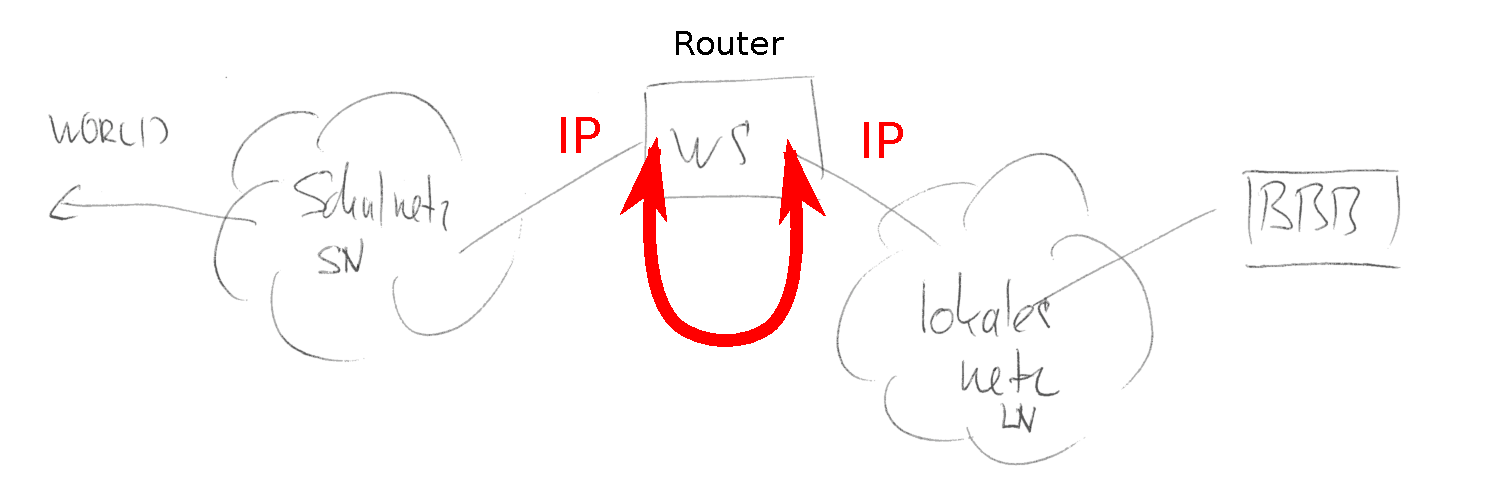
\includegraphics[width=0.875\textwidth]{router.pdf}
 \end{center}
 \begin{itemize}
  \item alle IP Protokolle 
  \item NAT Network Address Translation
 \end{itemize}
\end{frame}

\subsection{Konfiguration}
\begin{frame}[fragile]{Konfiguration}{\host}
  \begin{itemize}
  \item \cod{tools/forwarding.sh}
  \end{itemize}
\end{frame}

\begin{frame}[fragile]{Konfiguration}{\target}
  \begin{itemize}
  \item Setze gateway:
  \begin{lstlisting}[language=bash]
route add default gw host-ip usb0
  \end{lstlisting}
  \begin{itemize}
  \item Test 
  \begin{lstlisting}[language=bash]
ping ip-of-google.ch  
  \end{lstlisting}
  \end{itemize}
  \item Setze DNS Server
  \begin{lstlisting}[language=bash]
cp config/resolv.conf /etc/resolv.conf}

  \end{lstlisting}
  \begin{itemize}
   \item Test 
   \begin{lstlisting}[language=bash]
ping www.google.ch 
   \end{lstlisting}
  \end{itemize}
  \end{itemize}
\end{frame}

\section{Bridge}
\begin{frame}{Bridge}
 \begin{center}
 
\includegraphics[width=0.5\textwidth]{bridge-picture.pdf}
 \end{center}
 \begin{itemize}
  \item {\em Bridge} wirkt wie ein {\em Interface} 
  \begin{itemize}
   \item hat eine IP-Adresse 
  \end{itemize}
  \item {\em Bridge} verbindet {\em Interface}'s {\bf IFC}
 \end{itemize}
\end{frame}

\begin{frame}{Bridge: \cod{brctl}}{Auf dem \host}

\end{frame}

\section{Wi-Fi}
\subsection{Kernel}

\begin{frame}{Kernel}{Konfiguration}
{\footnotesize
 \dirtree{%
 .1 Kernel Configuration.
 .2 Networking support.
 .3 Wireless.
 .4 <*> cfg80211 - wireless configuration API.
 .4 <*> Generic IEEE 802.11 Networking Stack (mac80211).
 .2 Device Drivers.
 .3 Network device support.
 .4 Wireless LAN.
 .5 <*> TI wl18xx support.
 .5 <*> TI wlcore SPI support.
 .5 <*> TI wlcore SDIO support.
 }
}
\vspace{-5mm}
\begin{block}{Resultate}
 \begin{itemize}
  \item \cod{dmesg | grep wl}
 \end{itemize}
\end{block}
\end{frame}

\begin{frame}{Firmware}{Weitere Konfiguration}
 {\footnotesize
 \dirtree{%
 .1 Kernel Configuration.
 .2 Device Drivers.
 .3 Generic Driver Options.
 .4 [*] Include in-kernel firmware blobs in kernel binary.
 }
}
\vspace{-5mm}

\begin{block}{Resultate}
 \begin{itemize}
  \item \cod{dmesg | grep wl}
  \item \cod{ip link set wlan0 up}
  \item \cod{iw wlan0 scan}
  \item Weitere Konfiguration
 \end{itemize}
\end{block}
\end{frame}

\subsection{Connect}
\begin{frame}[fragile]{wpa}
 \begin{itemize}
  \item \cod{wpa\_passphrase}
  \item eduroam Versuch
{\footnotesize
\begin{verbatim}
network={
  ssid="eduroam"
  key_mgmt=WPA-EAP
  identity="hans.buchmann@fhnw.ch"
  domain_suffix_match="welcome.fhnw.ch"
  phase2="auth=MSCHAPV2"
  password="----"
}
\end{verbatim}
}
 \end{itemize}
\end{frame}

\begin{frame}[fragile]{DHCP}
 \begin{block}{manuell}
  \begin{itemize}
   \item \cod{udhcpc -v -i wlan0}
   \item \cod{ifconfig wlan0 {\em ip}}
   \begin{itemize}
    \item \cod{\em ip} abgelesen von \cod{udhcpc -v -i wlan0}
   \end{itemize}
  \end{itemize}
 \end{block}
 \begin{block}{automatisch/callback}
\vspace{-3mm}
{\tiny
\begin{verbatim}
#!/bin/sh
#---------------------
#on-udhcpc.sh
#(c) H.Buchmann FHNW 2017
#---------------------
case ${1} in
 defconfig)
  echo defconfig------- ${interface} ${ip};;
  bound)
   ifconfig ${interface} ${ip};;
esac
\end{verbatim}
}
\end{block}
\end{frame}

\begin{frame}{route/dns}
\begin{itemize}
 \item route
 \begin{itemize}
  \item \cod{route add default gw {\em gw-ip} wlan0}
 \end{itemize}
 \item DNS
 \begin{itemize}
   \item \cod{/etc/resolv.conf}
 \end{itemize}
\end{itemize}
\end{frame}



\section{Aufgaben}
\subsection{Proxy}

\begin{frame}{Aufgaben}{Proxy}
 \begin{itemize}
  \item Installiere Proxy
  \item Teste Proxy 
  \item Was wird auf den lokalen Netz übertragen 
  \begin{itemize}
   \item \cod{wireshark}
  \end{itemize}
  \item Setze \cod{apt-get} \& Co. so auf, dass \target per Internet/Proxy funktioniert 
 \end{itemize}
\end{frame}

\subsection{Forwarding}

\begin{frame}{Aufgaben}{Forwarding}
 \begin{itemize}
  \item Setze \host auf
  \item Setze \target auf
  \item Teste mit \cod{ping}
  \item Test mit \cod{apt-get}
 \end{itemize}
\end{frame}

\subsection{Wi-Fi}
\begin{frame}{Aufgaben}{Wi-Fi}
 \begin{itemize}
  \item setze Wi-Fi für eduroam auf
  \item Teste mit \cod{ping}
  \item Test mit \cod{apt-get}
 \end{itemize}
\end{frame}

\end{document}

